\section{Sewer interconnection}\label{se:sewer_interconnection}
This section will explain how pipes are interconnected and how the concentration for two joint pipes are calculated.

In figure \ref{fig:interconnections} an illustration of two pipes that are connected to the same point.

\begin{figure}[H]
\centering
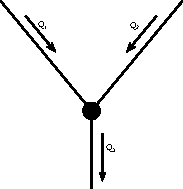
\includegraphics[width=0.30\textwidth]{report/modeling/pictures/interconnections}
\caption{Illustration of an interconnection between two flow inputs and one output.}
\label{fig:interconnections}
\end{figure} 

The two pipes leading into the point are connected, where the wastewater from the two pipes will be added up and transferred to the following pipe. The flow $Q_3$ is calculated as:

\begin{equation}
	\boxed{Q_3 = Q_1 + Q_2}
\end{equation} 

Which is a sum of the flows going into the point.

To calculate the concentration in a interconnection the following equation is used: %For the mixing between two flows where one of them is transporting chemicals will be done in similar way as for flows. 

\begin{equation}\label{poop_addition_interconnection}
	\boxed{C_3 = \frac{C_1 Q_1 + C_2 Q_2}{Q_3}}
\end{equation}

Where $C_1$ and $C_2$ is the amount of concentrate in the respective pipe $\left[g /m^3 \right]$. 


%This is done to keep the same amount of concentrate within the wastewater, as the algorithm for transporting concentrate depends on flow, as seen in section \ref{se:transport_of_concentrate}. %If it is not calculated like this, thus when the flow is increasing the same will the chemicals within the wastewater, hence it is needed to divided by $Q_3$ to get the right amount of chemicals in the wastewater.  